\section{Durchführung}
\label{sec:Durchführung}
\subsection{Versuchsaufbau}
Ein Schema des Aufbaus ist in Abbildung \ref{fig:Aufbau} zu sehen.
Das verwendete Licht wir von einer Rubidium-Spektrallampe bereitgestellt und mithilfe einer Sammellinse parallelisiert. Anschließend fällt das Licht auf einen Filter, welcher nur die D1-Spektrallinie transmittiert. Um das Licht rechtszirkular zu polarisieren wird es zunächst durch einen Linearpolarisator und anschließend durch ein $\frac{\lambda}{4}$-Plättchen gelenkt. Daraufhin fällt das Licht auf eine Dampfzelle, welche den Rubidiumdampf enthält. Der Dampf wird auf ca. $\SI{50}{\celsius}$ geheizt, wodurch eine breite Energieverteilung und ein konstanter Druck gewähleistet wird.
\begin{figure}[H]
  \centering
  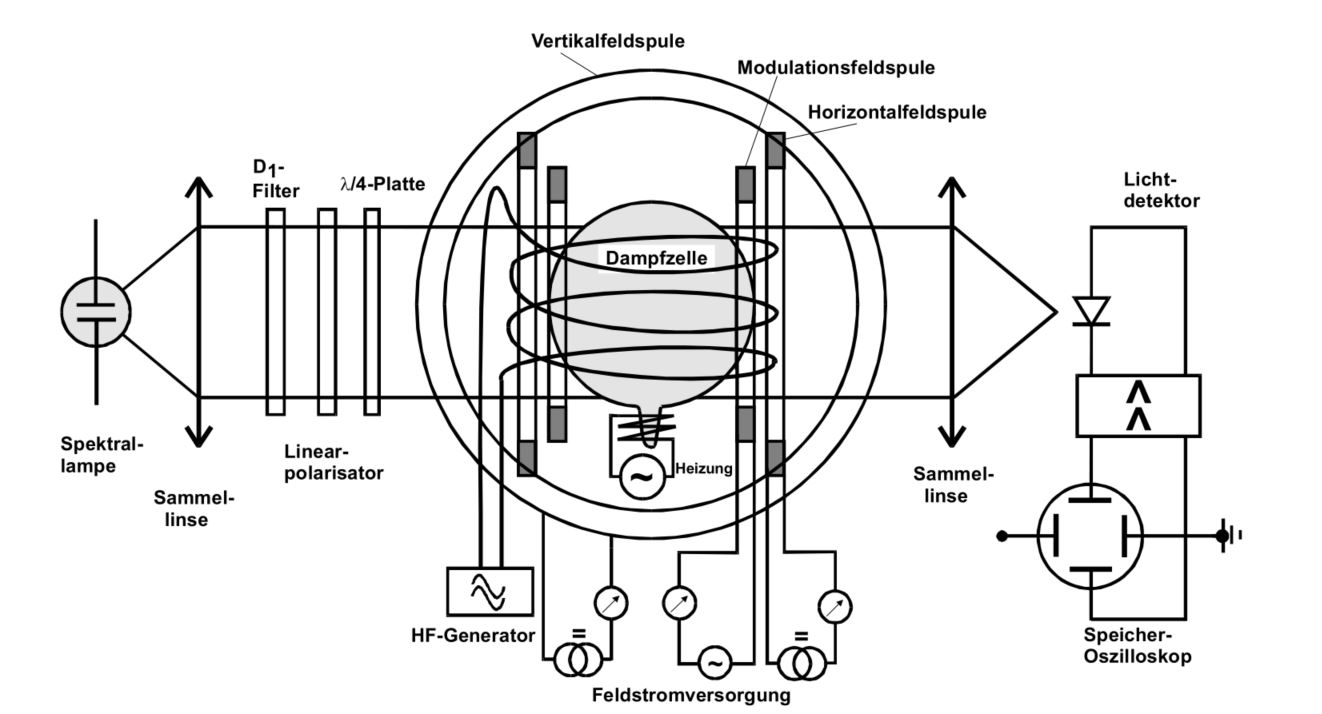
\includegraphics[width=\textwidth]{plots/Aufbau.JPG}
  \caption{Schematische Darstellung der zur Messung verwendeten Apparatur\cite{Anleitung}.}
  \label{fig:Aufbau}
\end{figure}
Die Dampfzelle befindet sich innerhalb der Felder dreier Helmholtzspulenpaare. Diese erzeugen ein horizontales und ein vertikales Magnetfeld sowie ein modulierbares Sweepfeld. Um die Dampfzelle ist ausserdem eine Hochfrequenzspule (RF-Spule) gewickelt.
Nachdem das Licht die Probenkammer passiert hat, wird es durch eine zweite Sammellinse auf einen Photodetektor fokussiert, dessen Ausgang an ein Oszilloskop angeschlossen wird.
\subsection{Versuchsdurchführung}
Damit auf der Photodiode möglichst viel Signal registriert wird muss die Apparatur zunächst so eingestellt werden, dass die Intensität des vermessenen Lichtes maximal ist. Dazu werden alle optischen Elemente ausser der Sammellinsen aus dem Strahlengang entfernt.
Die Sammellinsen werden nun so in den Strahlengang gebracht, dass die Brennpunkte sich in der Spektrallampe bzw. der Photodiode befinden.\\
Die Feldstärken der verwendeten Spulen liegen in der Größenordnung nahe der Feldstärke des Erdmagnetfeldes.
Um die dadurch entstehenden Auswirkungen möglichst einfach kompensieren zu können, wird mithilfe eines Helmholtzspulenpaares der vertikale Anteil des Erdmagnetfeldes kompensiert. Das auf dem Oszilloskop sichtbare Signal der Form \ref{fig:transfeld} (ohne den Resonanzpeak) wird nun mithilfe des Vertikalfeldes so moduliert, das der Peak bei Null eine möglichst geringe Breite aufweist. Außerdem wird die Apparatur so ausgerichtet, dass der Strahlengang parallel zur Nord-Süd-Richtung geführt ist. Dadurch geht nurnoch das horizontale Erdmagnetfeld als konstante Verschiebung in die Messungen ein. Abschließend wird der Aufbau durch eine schwarze Stoffdecke abgeschirmt um äußere Lichteinflüsse zu minimieren.\\
Die Hochfrequenzspule erzeugt aus einer Sinusspannung ein elektromagnetisches Wechselfeld, welches die Photonen zur induzierten Emission bereit stellt. Das Horizontalfeldspulenpaar erzeugt ein horizontales Magnetfeld, durch das die Zeeman-Aufspaltung ensteht. Mithilfe der Sweepspulen wird ein zweites, variables Magnetfeld erzeugt, welches das erste Horizontalfeld überlagert. Dieses Feld kann nun um die Null verfahren werden um die Transparenzkurve (wie in Abbildung \ref{fig:transfeld}) zu erzeugen.\\
Es werden bei unterschiedlichen Frequenzen des RF-Feldes die auf dem Oszilloskop sichtbaren Resonanzmagnetfelder $B_m$ in der Tanzparenzkurve vermessen.
